\documentclass[a4paper, 12pt]{article}
\usepackage[T2A]{fontenc}
\usepackage[utf8] {inputenc}
\usepackage[english, russian] {babel}
\usepackage{indentfirst}
\usepackage{amsmath}
\usepackage{amsfonts}
\usepackage{amssymb}
\usepackage{soulutf8}

\usepackage{geometry}
\geometry{left=2cm}
\geometry{right=1.5cm}
\geometry{top=1cm}
\geometry{bottom=2cm}

\usepackage{fancyhdr}
\pagestyle{fancy}
\fancyhead{}
\fancyhead[R]{\thepage}
\fancyhead[L]{\textit{Особенности решений уравнений теплопроводности с отклоняющимся аргументом}}
\setlength{\headheight}{48pt}
\fancyfoot{}

\begin{document}
\begin{center}
\textsc{\Huge{Особенности решений уравнений теплопроводности с отклоняющимся аргументом\\}}
\end{center}

\section{Постановка задачи, используемые допущения и вывод исследуемоего на устойчивость дифференциального \\уравнения}

Запишем \textbf{общее уравнение непрерывности} в дифференциальной форме:

\begin{equation}\label{eq:main}
\rho_t + div \bar{J} = f
\end{equation}

Оно представляет собой сильную (локальную) форму закона сохранения.

Рассмотрим случай, когда плотность потока будет выражена через плотность заряда следующим образом:

\begin{equation}
\bar{J} = -a^2 \nabla \rho + \bar{V} \rho
\end{equation}

Рассмотрим возмущенную систему, где $\tau$ \--- малый параметр:

\begin{equation}\label{eq:sys}
\bar{J}(x,t+\tau) = -a^2 \nabla \rho(x,t) + \bar{V}(x,t) \rho(x,t)
\end{equation}

\so{\textbf{Определение 1}}. Если в уравнении \ref{eq:sys}
\begin{enumerate}
\item $\tau>0$, то назовем его \textbf{уравнением с запаздывающим аргументом}
\item $\tau=0$, \--- \textbf{уравнением нейтрального типа}
\item $\tau<0$, \--- \textbf{уравнением опережающего типа}
\end{enumerate}

Разложим левую часть данного уравнения в ряд Тэйлора до члена порядка $m$:

\begin{equation*}
\bar{J}(x,t) + \bar{J_t}(x,t) \tau + \dots \dfrac{\partial^m \bar{J}}{\partial t^m}(x,t) \dfrac{\tau^m}{m!} = -a^2 \nabla \rho(x,t) + \bar{V}(x,t) \rho(x,t)
\end{equation*}

\begin{equation}\label{eq:sub}
\sum\limits_{k=0}^{m} \dfrac{\partial^k \bar{J}}{\partial t^k}(x,t) \dfrac{\tau^k}{k!} = -a^2 \nabla \rho(x,t) + \bar{V}(x,t) \rho(x,t)
\end{equation}

Продифференцировав исходное уравнение \ref{eq:main} $k$ раз, получим

\begin{equation*}
\dfrac{\partial^{k+1} \rho}{\partial t^{k+1}} + div \dfrac{\partial^k \bar{J}}{\partial t^k} = \dfrac{\partial^k f}{\partial t^k}
\end{equation*}

Домножив последнее уравнение на $\frac{\tau^k}{k!}$, перепишем его в следующем виде:

\begin{equation}\label{eq:div}
div \left( \dfrac{\partial^k \bar{J}}{\partial t^k} \right) \dfrac{\tau^k}{k!} = \left(\dfrac{\partial^k f}{\partial t^k} - \dfrac{\partial^{k+1} \rho}{\partial t^{k+1}} \right) \dfrac{\tau^k}{k!}
\end{equation}

Из уравнения \ref{eq:sub}:

\begin{equation*}
\sum\limits_{k=0}^{m} div \left(\dfrac{\partial^k \bar{J}}{\partial t^k} \right) \dfrac{\tau^k}{k!} = -a^2 div(\nabla \rho) + div(\bar{V} \rho)
\end{equation*}

Подставим \ref{eq:div}:

\begin{equation*}
\sum\limits_{k=0}^{m} \left(\dfrac{\partial^k f}{\partial t^k} - \dfrac{\partial^{k+1} \rho}{\partial t^{k+1}} \right) \dfrac{\tau^k}{k!} = - a^2 \Delta \rho + \rho div\bar{V} + (\bar{V},\nabla \rho)
\end{equation*}

\begin{equation*}
\sum\limits_{k=0}^{m} \dfrac{\partial^{k+1} \rho}{\partial t^{k+1}} \dfrac{\tau^k}{k!} - a^2 \Delta \rho + \rho div\bar{V} + (\bar{V},\nabla \rho) = \sum\limits_{k=0}^{m} \dfrac{\partial^k f}{\partial t^k} \dfrac{\tau^k}{k!}
\end{equation*}

Рассмотрим одномерный случай:

\begin{equation*}
\sum\limits_{k=0}^{m} \dfrac{\partial^{k+1} \rho}{\partial t^{k+1}} \dfrac{\tau^k}{k!} - a^2 \dfrac{\partial^2 \rho}{\partial x^2} + \rho \dfrac{\partial V}{\partial x} + V \dfrac{\partial \rho}{\partial x} = \sum\limits_{k=0}^{m} \dfrac{\partial^k f}{\partial t^k} \dfrac{\tau^k}{k!} = g(x,t)
\end{equation*}

Для простоты примем $g=0$ и $V=const$:

\begin{equation}
\sum\limits_{k=0}^{m} \dfrac{\partial^{k+1} \rho}{\partial t^{k+1}} \dfrac{\tau^k}{k!} - a^2 \dfrac{\partial^2 \rho}{\partial x^2} + V \dfrac{\partial \rho}{\partial x} = 0
\end{equation}

Заменим неизвестную функцию следующим образом:

\begin{equation*}
\rho (x,t) = e^{\xi x} u(x,t)
\end{equation*}

Тогда

\begin{align*}
\rho_x & = e^{\xi x} (u_x + \xi u)\\
\rho_{xx} & = e^{\xi x} (u_{xx} + 2 \xi u_x + \xi^2 u)
\end{align*}

\begin{align*}
- a^2 \rho_{xx} + V \rho_x = e^{\xi x} \lbrack -a^2 (u_{xx} + 2 \xi u_x + \xi^2 u) + V (u_x + \xi u) \rbrack = \\
= e^{\xi x} \lbrack -a^2 u_{xx} + (-2 a^2 \xi + V) u_x + (-a^2 \xi^2 + V \xi) u \rbrack = \\
= e^{\xi x} \left\lbrack -a^2 u_{xx} + \dfrac{V^2}{4a^2} u \right\rbrack
\end{align*}

при $\xi = \frac{V}{2a^2}$ (т.е. коэффициент при $u_x$ равен $0$).

Наконец, получим уравнение, для которого будем исследовать устойчивость его решений:

\begin{equation}\label{eq:final}
\sum\limits_{k=0}^{m} \dfrac{\partial^{k+1} u}{\partial t^{k+1}} \dfrac{\tau^k}{k!} - a^2 \dfrac{\partial^2 u}{\partial x^2} + \dfrac{V^2}{4a^2} u = 0
\end{equation}
\section{Исследование устойчивости исходного уравнения в частных производных}

\subsection{Метод Фурье для исходного уравнения}

Для уравнения \ref{eq:final} применим \textbf{метод Фурье разделения переменных}:

\begin{equation*}
u(x,t) = T(t) X(x)
\end{equation*}

\begin{equation*}
\sum\limits_{k=0}^{m} \dfrac{\tau^k}{k!} T^{(k+1)} X + \dfrac{V^2}{4a^2} T X =a^2 T X''
\end{equation*}

\begin{equation*}
\dfrac{\sum\limits_{k=0}^{m} \dfrac{\tau^k}{k!} T^{(k+1)} + \dfrac{V^2}{4a^2} T}{a^2 T} = \dfrac{X''}{X} = -\lambda = -k^2
\end{equation*}

\begin{equation}
\left\{
\begin{aligned}
\sum\limits_{k=0}^{m} \dfrac{\tau^k}{k!} T^{(k+1)} + \underbrace{ \left( \dfrac{V^2}{4a^2} + a^2 k^2 \right)}_{\gamma} T & = 0\\
X'' + k^2 X & = 0
\end{aligned}
\right.
\end{equation}

Как видно, малый параметр входит только в уранение относительно $T(t)$.

Целью нашего дальнейшего исследования является обосновать устойчивость или неустойчивость решений 

\begin{equation*}
\sum\limits_{k=0}^{m} \dfrac{\tau^k}{k!} T^{(k+1)} + \underbrace{ \left( \dfrac{V^2}{4a^2} + a^2 k^2 \right)}_{\gamma} T = 0
\end{equation*}

при различных $m$.

\subsection{Исследование устойчивости обыкновенного дифференциального уравнения относительно $T(t)$}

Напомним, что в данном пункте исследуется уравнение 

\begin{equation*}
\sum\limits_{k=0}^{m} \dfrac{\tau^k}{k!} T^{(k+1)} + \underbrace{ \left( \dfrac{V^2}{4a^2} + a^2 k^2 \right)}_{\gamma} T = 0
\end{equation*}

Выпишем характеристическое уравнение:

\begin{equation*}
\sum\limits_{k=0}^{m} \dfrac{\tau^k}{k!} \lambda^{k+1} + {\gamma} = 0
\end{equation*}

Согласно общей теории, для алгебраического уравнения

\begin{equation}\label{eq:alg}
a_0 x^n + a_1 x^{n-1} + \dots + a_{n-1} x + a_n = 0 \quad a \neq 0
\end{equation}

выполнена

\so{\textbf{Теорема Рауса-Гурвица}}. Число корней с положительной частью действительного алгебраического уравнения \ref{eq:alg} равно числу перемен знака в любой из последовательностей

\begin{equation*}
T_0, T_1, \dfrac{T_2}{T_1}, \dots, \dfrac{T_n}{T_{n-1}}
\end{equation*}

или

\begin{equation*}
T_0, T_1, T_1 T_2, T_2 T_3, \dots, T_{n-2} T_{n-1}, a_n
\end{equation*}

где

\begin{align*}
& T_0 = a_0 > 0, \quad T_1 = a_1, \quad T_2 = 
\begin{pmatrix}
a_1 & a_0\\
a_3 & a_2
\end{pmatrix},\\
& T_3 = 
\begin{pmatrix}
a_1 & a_0 & 0\\
a_3 & a_2 &a_1\\
a_5 & a_4 &a_3
\end{pmatrix}, \quad T_4 =
\begin{pmatrix}
a_1 & a_0 & 0 & 0\\
a_3 & a_2 & a_1 & a_0\\
a_5 & a_4 & a_3 & a_2\\
a_7 & a_6 & a_5 & a_4
\end{pmatrix}, \dots
\end{align*}

\so{\textbf{Критерий Рауса-Гурвица}}. Для того, чтоюы все корни действительного уравнения \ref{eq:alg} имели отрицательные действительные части необходимо и достачно, чтобы выполнялись неравенства:

\begin{equation*}
T_0 > 0, T_1 >0, \dots, T_n > 0
\end{equation*}

Отметим, что согласно построению, можем считать $\gamma(k) ~ k^2$ неограниченным, а $\tau > 0$ зафиксировать.

Таким образом, задача об устойчивости решений дифференцаильного уравнения относительно $T(t)$ сводится к нахождению определителей матриц Гурвица для различных $m$.

Вычислим их програмно, где числовые коэффициенты запишем в десятичной форме,

\textbf{при $m=1$}: $T_1 = 1 > 0$, $T_1 = \gamma > 0$\\

\textbf{при $m=2$}: $T_1 = \tau$, $T_2 = \tau (1 - 0.5 \gamma \tau) < 0$, $T_3 = \gamma \tau (1 - 0.5 \gamma \tau) < 0$\\

\textbf{при $m=3$}: $T_1 = 0.5 \tau ^2$, $T_2 = 0.333333 \tau ^3$, $T_3 = \tau ^3 (0.333333\, -0.25 \gamma  \tau ) < 0$, $T_4 = \gamma  \tau ^3 (0.333333\, -0.25 \gamma  \tau ) < 0$\\

\textbf{при $m=4$}: $T_1 = 0.167 \tau ^3$, $T_2 = 0.041 \tau ^5$, $T_3 = \tau ^6 (0.007 \gamma  \tau + 0.014)$, \\$T_4 = \tau ^6 \left(-0.0017 \gamma ^2 \tau ^2-0.007 \gamma  \tau +0.014\right) < 0$, $T_5 = \gamma  \tau ^6 \left(-0.0017 \gamma ^2 \tau ^2-0.0071 \gamma  \tau +0.0139 \right)$\\

\textbf{при $m=5$}: $T_1 = 0.042 \tau ^4$, $T_2 = 0.003 \tau ^7$, $T_3 = 0$, $T_4 = \tau ^{10} (0.0001 \gamma  \tau -0.0002)$, $T_5 = \tau ^{10} \left(-0.0001 \gamma ^2 \tau ^2+0.0002 \gamma  \tau -0.0002\right) < 0$, \dots\\

\textbf{при $m=6$}: $T_1 = 0.0083 \tau ^5$, $T_2 = 0.0001 \tau ^9$, $T_3 = -3.858^{-6} \tau ^{12} < 0$, \dots\\

\textbf{при $m=7$}: $T_1 = 0.00138889 \tau ^6$, $T_2 = 3.307^{-6} \tau ^{11}$, $T_3 = -4.593^{-8} \tau ^{15} < 0$, \dots\\

Отметим, что $T_3$, начиная с того момента, когда не зависит от $\gamma$ (т.е. при $m \geq 6$), отрицательны при $\tau>0$ для приведенных $m$

\so{\textbf{Утверждение}}. $T_3 < 0$ при $m \geq 6$.

Выпишем общий вид определителя матрицы Гурвица при $k=3$:

\begin{equation*}
T_3 = 
\begin{vmatrix}
\frac{\tau^{m-1}}{(m-1)!} & \frac{\tau^{m}}{m!} & 0\\
\frac{\tau^{m-3}}{(m-3)!} & \frac{\tau^{m-2}}{(m-2)!} & \frac{\tau^{m-1}}{(m-1)!}\\
\frac{\tau^{m-5}}{(m-5)!} & \frac{\tau^{m-4}}{(m-4)!} & \frac{\tau^{m-3}}{(m-3)!}
\end{vmatrix} =
\dfrac{\tau^{m-1}}{(m-1)!}
\begin{vmatrix}
\frac{\tau^{m-2}}{(m-2)!} & \frac{\tau^{m-1}}{(m-1)!}\\
\frac{\tau^{m-4}}{(m-4)!} & \frac{\tau^{m-3}}{(m-3)!}
\end{vmatrix}
- \dfrac{\tau^{m}}{m!}
\begin{vmatrix}
\frac{\tau^{m-3}}{(m-3)!} & \frac{\tau^{m-1}}{(m-1)!}\\
\frac{\tau^{m-5}}{(m-5)!} & \frac{\tau^{m-3}}{(m-3)!}
\end{vmatrix}
\end{equation*}

\begin{equation*}
T_3 =
\dfrac{\tau^{m-1}}{(m-1)!} \dfrac{\tau^{m-2}}{(m-2)!} \dfrac{\tau^{m-4}}{(m-4)!}
\begin{vmatrix}
1 & \frac{\tau}{m-1}\\
1 & \frac{\tau}{m-3}
\end{vmatrix}
- \dfrac{\tau^{m}}{m!} \dfrac{\tau^{m-3}}{(m-3)!} \dfrac{\tau^{m-5}}{(m-5)!}
\begin{vmatrix}
1 & \frac{\tau^2}{(m-2)(m-1)}\\
1 & \frac{\tau^2}{(m-4)(m-3)}
\end{vmatrix}
\end{equation*}

\begin{multline*}
T_3 = \dfrac{\tau^{3m-7}}{(m-1)!(m-2)!(m-4)!} \left( \dfrac{\tau}{m-3} - \dfrac{\tau}{m-1} \right) \\ - \dfrac{\tau^{3m-8}}{m!(m-3)!(m-5)!} \left( \dfrac{\tau^2}{(m-4)(m-3)} - \dfrac{\tau^2}{(m-2)(m-1)} \right)
\end{multline*}

\begin{multline*}
T_3 = \tau^{3m-6} \left( \dfrac{(m-1) - (m-3)}{(m-1)!(m-2)!(m-4)!(m-3)(m-1))} \right. \\ \left. - \dfrac{(m-2)(m-1) - (m-4)(m-3)}{m!(m-3)!(m-5)!(m-4)(m-3)(m-2)(m-1)} \right)
\end{multline*}

\begin{equation*}
T_3 = \dfrac{\tau^{3m-6}}{m!(m-1)!(m-3)!} (2m - (-3m + 2 + 7m - 12)) = \dfrac{\tau^{3m-6}}{m!(m-1)!(m-3)!} (10-2m) < 0
\end{equation*}

при $m \geq 6$.

Построим график для значений $T_3$ в зависимости от $m$:

\begin{center}
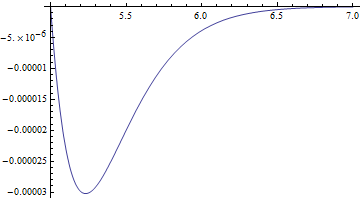
\includegraphics[width=0.5\textwidth]{coefCheck.png}
\end{center}

Таким образом, решение исходной задачи устойчиво только при $m=1$.
\end{document}